\part{Teoría del Caos}
\section{Atractor de Lorentz}
Como una cuestión previa conviene aclarar conceptos porque tiende a confundirse Caos y Fractales (ver figura \ref{img:fibo}). En artículos de divulgación y en muchas publicaciones vienen juntos y mezclados, por lo que hay que precisar que Caos y Fractales no son sinónimos y tienen comportamientos distintos a pesar de compartir una formulación sencilla y que ciertos fenómenos caóticos tengan una estructura fractal como es el caso del atractor de Lorenz que podemos observar en la figura \ref{img-lorentz} visto en la pagina \pageref{img-lorentz}.
\begin{figure}[H]
	\centering
	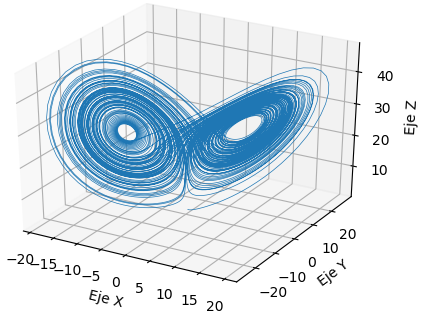
\includegraphics[scale=0.8]{img/tlorentz}
	\caption{Atractor de Lorentz}
	\label{img-lorentz}
\end{figure}
Los estudios de Edward Lorenz sobre  "Dependencia sensitiva de las condiciones iniciales" y el famoso efecto mariposa son el origen de la Teoría del Caos.
\begin{figure}[H]
	\centering
	\caption{Fractal de Fibonacci. Fuente: \url{https://rosettacode.org/wiki/Fibonacci_word/fractal}}
	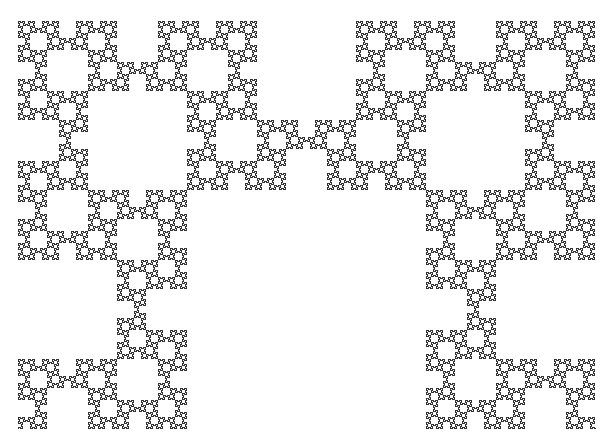
\includegraphics[scale=0.6]{img/fractal}
	\label{img:fibo}
\end{figure}
El término atractor extraño se debe a David Ruelle y Floris Takens, físico-matemático el primero y matemático el segundo. Lo definieron como: una zona bien delimitada del espacio de fases en la que las líneas de la trayectoria del sistema nunca se cortan. Líneas de longitud infinita confinadas en área finita, describiendo órbitas no periódicas. Ni Ruelle ni Takens lo habían visto nunca, pero presagiaron su existencia. Ese monstruo matemático, según ellos, debería de ser fractal.

\begin{figure}[H]
	\centering
	\subfigure[Primera figura]{
		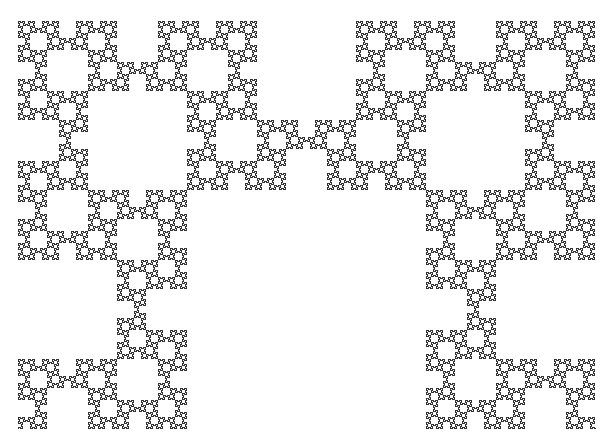
\includegraphics[scale=0.3]{img/fractal}}
		\quad
	\subfigure[Segunda figura]{
		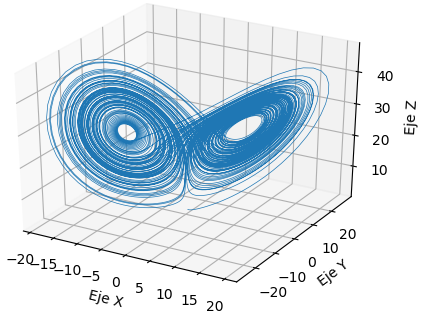
\includegraphics[scale=0.4]{img/tlorentz}}
	\caption{Gráficas importantes en la teoria del caos}
\end{figure}

Sea la tabla \ref{tb:implementos} podemos observar los implementos necesarios para poder restaurar nuestro laboratorio de Química General.

\begin{table}[h]
\begin{center}
\caption{}
	\begin{tabular}{| c | c | c | c |}
		\hline
		\multicolumn{4}{| c |}{Instrumentos} \\ \hline
		\multicolumn{2}{| c |}{Items} & \multicolumn{2}{| c |}{Inventario} \\ \hline
		\bf Materiales & \bf Precio & \bf Cantidad & \bf Salón \\ \hline
		Probeta & 70 & 5 & KFC-1\\
		Matraz & 26 & 13 & KFC-2\\
		Pipeta & 30 & 3 & KFC-3\\ \hline
	\end{tabular}\\
	\normalsize{Implementos para un laboratorio de Química I}
	\label{tb:implementos}
\end{center}
\end{table}

\section{Exponente de Lyapunov}
\begin{multicols}{2}
El Exponente Lyapunov o Exponente característico Lyapunov de un sistema dinámico es una cantidad que caracteriza el grado de separación de dos trayectorias infinitesimalmente cercanas. Cuantitativamente, dos trayectorias en el espacio-fase con separación inicial $\delta Z_0$ diverge.

El radio de separación puede ser distinto para diferentes orientaciones del vector de separación inicial.\columnbreak

Aunque, hay un completo espectro del exponente Lyapunov; el número de ellos es igual al número de dimensiones del espacio-fase. Es común referirse sólo a la más grande, porque determina la predictibilidad de un sistema.
Los exponentes característicos de Lyapunov (LCE del inglés Lyapunov Characteristic Exponents) son una herramienta que permite cuantificar la velocidad a la que se separan dos órbitas con condiciones iniciales infinitamente cercanas. Por ello, con frecuencia se emplean como indicadores de la presencia de caos.
\end{multicols}